\documentclass[sigconf]{acmart}

\AtBeginDocument{%
  \providecommand\BibTeX{{%
    Bib\TeX}}}

\usepackage{listings}
\lstset{
  basicstyle=\footnotesize\ttfamily,
  keywordstyle=\bfseries,
  commentstyle=\itshape\color{gray},
  breaklines=true,
  frame=single,
  numbers=none,
  xleftmargin=2pt,
  xrightmargin=2pt,
}

\setcopyright{none}
\acmConference{}{}{}
\acmBooktitle{}
\acmDOI{}
\acmISBN{}
\settopmatter{printacmref=false, printfolios=true}
\fancyfoot{}

\begin{document}

\title{Structured AI Theorem Proving with Human-Learnable Knowledge Extraction}

\author{Zihan Zheng}
\affiliation{%
  \institution{University of Illinois Urbana-Champaign}
  \country{USA}}
\email{zihanz23@illinois.edu}

\author{Author Two}
\affiliation{%
  \institution{University of Illinois Urbana-Champaign}
  \country{USA}}
\email{author2@illinois.edu}

\author{Author Three}
\affiliation{%
  \institution{University of Illinois Urbana-Champaign}
  \country{USA}}
\email{author3@illinois.edu}

\author{Author Four}
\affiliation{%
  \institution{University of Illinois Urbana-Champaign}
  \country{USA}}
\email{author4@illinois.edu}

\begin{abstract}
As AI systems increasingly generate formal proofs and complex code artifacts, a critical gap emerges: the proof is verified, but human understanding lags behind. A verified theorem tells us \emph{what} is true, not \emph{why} it is true, \emph{when} the technique applies, or \emph{what} we should learn from it. We present a two-system architecture for Lean~4 theorem proving that addresses this gap. System~1 is a structured prover that separates high-level mathematical strategy from low-level mechanization through a plan--implement--replan loop with proof skeletons. System~2 is a digest agent that extracts transferable, human-learnable knowledge from proving traces via reinterpretation, scope expansion, progressive construction, and strategy templates. We evaluate against a curated dataset derived from a 455-node, 1596-edge mathematical knowledge graph with human-authored reasoning. Preliminary results on a complex subset sum case study show that 100\% of proving errors are mechanization (wrong API names, syntax), not mathematical strategy, validating the separation. The digest agent recovers 100\% of ground-truth strategy connections versus 50\% for a baseline summarizer.
\end{abstract}

\maketitle

\section{Problem}
The classification of finite simple groups took 50 years, 500 papers, and 15,000 pages. The ``simplified'' GLS project, begun in 1981, has published 9 of 12 planned volumes and is still ongoing. The proof exists; the understanding lags decades behind. Now imagine an AI system produces a Lean-verified proof of a significant conjecture---the compiler says \checkmark, but what has humanity actually learned? This concern extends beyond mathematics: an AI-generated 10,000-line GPU kernel that runs 5$\times$ faster gives us a faster kernel, but the engineer who reads it cannot extract the principles that would make them better at writing kernels.

We identify two core problems with current LLM-based theorem proving systems:

\paragraph{Verified $\neq$ Understanding.}
Current systems optimize for one metric---does the proof compile?---and discard everything else. The proving process (what was tried, what failed, what the exploration revealed) is thrown away. Only the final artifact survives. A student reading an AI-generated Lean proof learns less than one who struggled through it. A researcher who receives an AI proof of their conjecture knows it is true but may not gain the insight needed for the next one.

\paragraph{Mechanization $\neq$ Reasoning.}
Current provers use a single model for everything: choosing the proof strategy, finding the right Mathlib lemma name, and fixing syntax errors. These are fundamentally different tasks. In our case study, 100\% of failed proving iterations were mechanization errors---wrong API names, predicate form mismatches, tactic scope issues---while the mathematical strategy was correct from the first attempt. A powerful reasoning model should not spend its capacity on whether Mathlib calls a lemma \texttt{Complex.norm\_eq\_abs} or \texttt{Complex.abs\_re\_le\_norm}; that is a retrieval problem, not a reasoning problem.

Our objective is to design a system whose proving process produces not only verified proofs but \emph{human-learnable} knowledge: what to avoid, why certain choices were made, what strategies transfer, and what the proof reveals about the structure of the problem.


\section{Solution}
We propose a two-system architecture (Figure~\ref{fig:arch}): a \textbf{prover agent} (System~1) that generates verified proofs through a structured loop, and a \textbf{digest agent} (System~2) that extracts human-learnable knowledge from the proving traces. Lessons from System~2 feed back into System~1 to improve future sessions. Our implementation targets Lean~4 with Mathlib, using an MCP server that exposes a \texttt{check\_lean\_proof} tool for compilation and diagnostics. Source code is available at \url{https://github.com/Ravencus/CS598LMZ-LEAN}.

\begin{figure}[h]
  \centering
  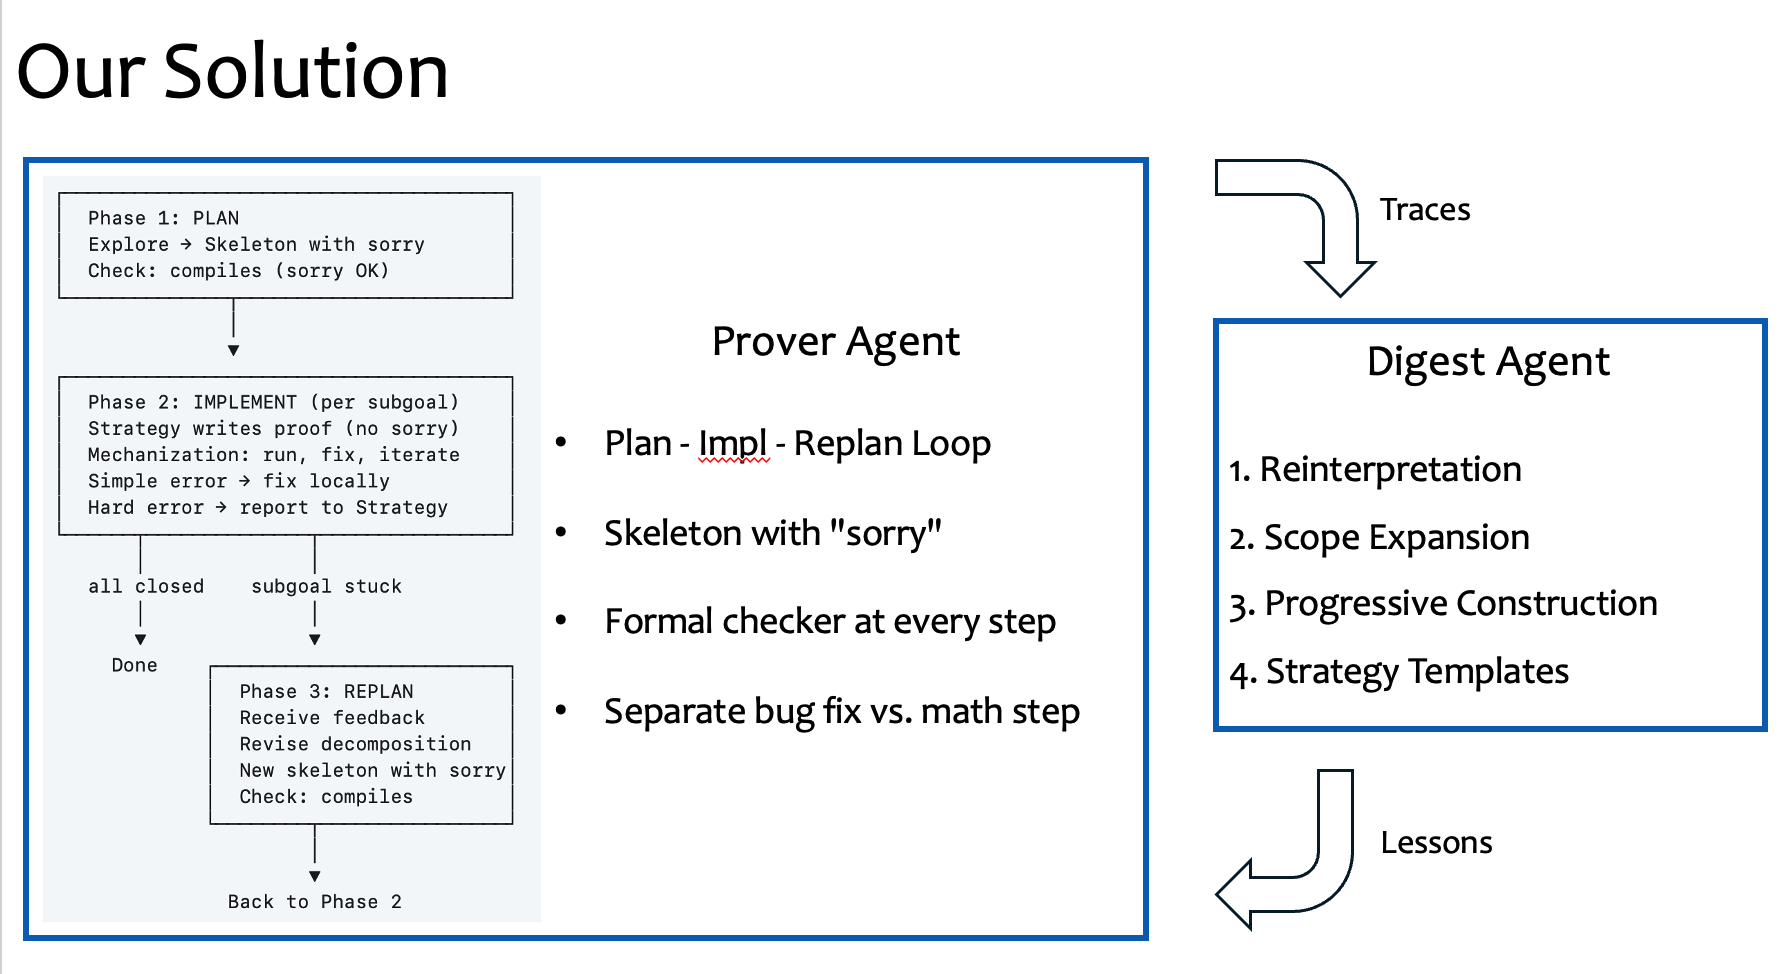
\includegraphics[width=\linewidth]{figures/architecture}
  \caption{Two-system architecture. The prover agent follows a plan--implement--replan loop with proof skeletons. Traces flow to the digest agent, which extracts lessons that feed back to future proving sessions.}
  \label{fig:arch}
\end{figure}

\subsection{System 1: Prover Agent}

The prover operates in three phases. In \textbf{Phase~1 (Plan)}, a strategy agent explores the problem and produces a proof skeleton---a complete Lean file where the main theorem is proved from sorry'd subgoals. The skeleton must compile (sorry warnings are acceptable, errors are not), validating that the decomposition is structurally sound. In \textbf{Phase~2 (Implement)}, each sorry'd subgoal is filled in. A mechanization agent (cheap model with many calls) handles simple compilation errors---wrong lemma names, type mismatches, predicate form issues---and only escalates to the strategy agent (powerful model, few calls) when the error requires mathematical insight. In \textbf{Phase~3 (Replan)}, if a subgoal fails repeatedly, the strategy agent receives structured feedback and revises the decomposition, producing a new skeleton.

\subsection{System 2: Digest Agent}

The digest agent takes a proving trace and performs four core functions that mirror how humans learn from problem-solving. \textbf{Reinterpretation} strips domain-specific surface to find the essential structure (e.g., ``complex numbers'' $\to$ 2D vectors and directional alignment). \textbf{Scope expansion} generates natural follow-up questions that deepen understanding beyond the stated goal (e.g., can we beat $1/6$? what is the optimal bound?). \textbf{Progressive construction} starts from the simplest non-trivial case and identifies what carries forward to the general case. \textbf{Strategy templates} extract high-level approaches and connections to other problems where similar strategies apply. The output is stored as standalone digests and lemma annotations with strategic context, both retrievable by the prover in future sessions.


\section{Evaluation Setup}
\subsection{Dataset Curation}

Our evaluation dataset is derived from a proprietary, human-authored Obsidian knowledge base of mathematical problem-solving notes (455 notes, 1596 bidirectional links). Unlike standard (problem, proof) datasets, each note contains the author's reasoning process: problem reinterpretation, technique identification, difficulty progression, and connections to related problems. The link structure encodes an explicit relational graph where a few high-level strategies (hub nodes) connect to many specific problems (leaf nodes), following a power-law degree distribution (Figure~\ref{fig:tiers}).

Raw notes require curation because one note may contain multiple problems (original, strengthened, generalized), and edges are at note level rather than problem level. Our pipeline has four steps: (1)~extract individual problem statements from each note, (2)~rebuild connections at the problem level (inherited edges from note-level links, internal edges from within-note progression), (3)~formalize each problem as a Lean~4 theorem statement with \texttt{sorry} and verify compilation, (4)~classify nodes into problem nodes (formalizable) and technique nodes (pure strategy descriptions). The 34 hub nodes (degree $\geq$10, 7\% of total) serve as ground-truth strategy labels for evaluation.

\begin{figure}[h]
  \centering
  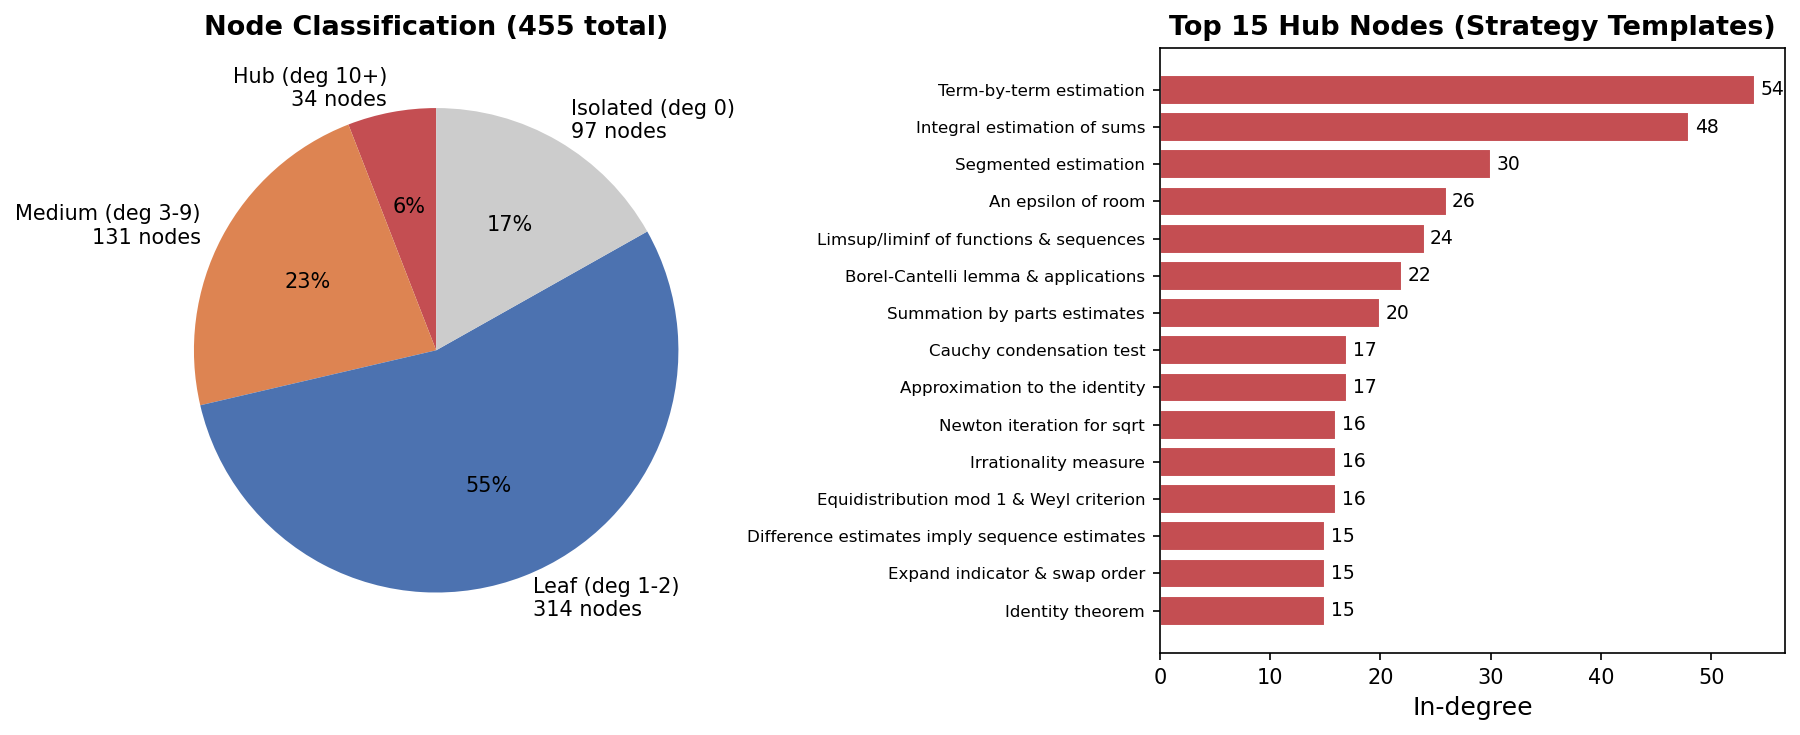
\includegraphics[width=\linewidth]{figures/tier-breakdown}
  \caption{Left: node classification by in-degree tier (455 total). Right: top 15 hub nodes representing reusable strategy templates.}
  \label{fig:tiers}
\end{figure}

\subsection{Evaluation 1: Prover Effectiveness}

We compare our structured workflow (plan--implement--replan with mechanization separation) against free agents (same model, same Lean checker MCP tool, no structured workflow). Baselines include Claude Code, OpenCode, and dedicated provers such as ReProver and Lean Copilot. Metrics: (1)~\textbf{Pass@k}---does the agent produce a sorry-free proof? (2)~\textbf{Iteration count}---how many LLM $\leftrightarrow$ Lean checker rounds? (3)~\textbf{Error type}---mechanization (wrong API name, syntax, type mismatch) versus mathematical (wrong strategy, dead-end decomposition).

\subsection{Evaluation 2: Knowledge Extraction Quality}

We evaluate whether the digest agent extracts deep, transferable knowledge or shallow summaries. The baseline is prompt-based summarization (``summarize the key ideas of this proof''). The setup: given a problem and its proof trace, the agent extracts lessons, which are then compared against ground-truth edges from the knowledge graph via semantic matching. Metrics: \textbf{precision} (of the connections the digest claims, how many match ground-truth edges?) and \textbf{recall} (of the ground-truth edges, how many does the digest recover?), weighted toward hub connections since recovering a link to a high-degree strategy template is more valuable than recovering a leaf-to-leaf connection.


\section{Result Analysis}
Our preliminary results are from a single case study---the complex subset sum problem: given $n$ complex numbers with $\sum\|z_k\| = 1$, prove there exists a subset $S$ with $\|\sum_{k\in S} z_k\| \geq c$. We formalized two proofs in Lean~4: the quadrant method ($c = 1/4$, fully verified) and the averaging method ($c = 1/\pi$, optimal bound, algebraic structure verified with 3 sorry's in the analytic core).

Figure~\ref{fig:skeleton} shows the proof skeleton for the averaging method. Phase~1 produces three sorry'd subgoals---a pure computation, a standard analysis result, and integration plumbing---while the main theorem is fully proved from them. The sorry's mark exactly where the math ends and the mechanization begins. The skeleton is also far more readable than the full $\sim$300-line proof.

\begin{figure}[h]
\begin{lstlisting}
-- Phase 1: Skeleton (sorry'd subgoals, compiles)

lemma integral_max_cos :          -- sorry: computation
  integral (0)..(2*pi),
    max (cos u) 0 = 2 := by sorry

lemma exists_ge_avg              -- sorry: library gap
  (h : integral f = C) :
  exists x, f x >= C/(b-a) := by sorry

lemma averaging_argument         -- sorry: plumbing
  (h : sum ||z_k|| = 1) :
  exists alpha, sum_{S_alpha}
    Re(z_k * exp(-i*alpha)) >= 1/pi
  := by sorry

-- Phase 2: Main theorem (no sorry)

theorem complex_subset_sum_pi
  (h : sum ||z_k|| = 1) :
  exists S, ||sum_{S} z_k|| >= 1/pi := by
  obtain <alpha_0, h_alpha> :=
    averaging_argument h
  exact <S_{alpha_0},
    le_trans h_alpha (norm_ge_proj ...)>
\end{lstlisting}
\caption{Proof skeleton for the $1/\pi$ bound. Sorry'd subgoals (Phase~1) validate the decomposition; the main theorem (Phase~2) is fully proved from them.}
\label{fig:skeleton}
\end{figure}

\subsection{Prover Results}

Table~\ref{tab:prover} summarizes the structured agent's performance. Across both proofs, the mathematical strategy was correct from the first attempt and never revised. All 36 checker calls were mechanization work.

\begin{table}[h]
  \caption{Prover results on complex subset sum (structured Opus 4.6).}
  \label{tab:prover}
  \small
  \begin{tabular}{lcccc}
    \toprule
    Proof & Calls & Math err. & Mech. err. & Revisions \\
    \midrule
    Quadrant ($1/4$) & 9 & 0 & 9 & 0 \\
    API search & 11 & --- & --- & --- \\
    Averaging ($1/\pi$) & 16 & 0 & 16 & 0 \\
    \midrule
    \textbf{Total} & \textbf{36} & \textbf{0} & \textbf{36} & \textbf{0} \\
    \bottomrule
  \end{tabular}
\end{table}

The error breakdown: $\sim$11 wrong Mathlib API names, $\sim$4 predicate form mismatches ($\geq 0$ vs.\ $0 \leq$), $\sim$8 tactic/expression rewrites, 11 API search calls (\texttt{exact?}, \texttt{\#check}), and 2 successful compilations. This validates the strategy/mechanization separation: a cheap model with Lean API knowledge could have handled all 34 non-final calls, reducing powerful-model usage by $\sim$95\%.

For the free agent baseline (same Opus 4.6 model, no structured workflow), the attempt failed after 25 minutes consuming 1M context tokens without producing a verified proof, underscoring the value of the structured plan--implement--replan loop.

\subsection{Knowledge Extraction Results}

The complex subset sum problem has two ground-truth hub connections in our knowledge graph: the probabilistic method (averaging argument) and the pigeonhole principle (quadrant/sector argument). Table~\ref{tab:digest} shows preliminary hub-recovery recall.

\begin{table}[h]
  \caption{Hub-recovery recall on complex subset sum (2 ground-truth hubs).}
  \label{tab:digest}
  \begin{tabular}{lcc}
    \toprule
    Agent type & Hubs recovered & Recall \\
    \midrule
    Prompt-based summary & 1/2 & 50\% \\
    Digest agent & 2/2 & 100\% \\
    \bottomrule
  \end{tabular}
\end{table}

The prompt-based baseline identified the pigeonhole connection but missed the probabilistic method. Our digest agent, through scope expansion (``can we beat $1/6$?'') and strategy templates, recovered both. This suggests the four core functions surface deeper structural connections that naive summarization misses.

\subsection{Limitations}

We identified a \textbf{data leakage concern}: Opus 4.6 recalled the optimal bound $1/\pi$ from training data rather than deriving it. The correct proof skeleton may reflect memorization, not reasoning. Even in this best case---memorized strategy---the agent still required 36 calls of mechanization overhead. With a smaller model or a novel problem, strategy errors would compound on top. Full-scale evaluation with diverse problems and models is needed to disentangle recall from reasoning.


\section{Future Plan}
\paragraph{Full-scale evaluation.} Run the prover and digest agent on many problems from the curated dataset across multiple models (Opus 4.6, GPT 5.4, smaller models via OpenCode). This will provide the replanning data and error breakdowns currently missing from our single-problem preliminary results, and test whether the strategy/mechanization separation holds across difficulty levels.

\paragraph{Dataset curation completion.} Finish extracting individual problems from the 455-note vault, formalizing each as a Lean~4 theorem statement, and rebuilding edges at the problem level. This unlocks the full evaluation pipeline.

\paragraph{CAS integration.} Add Mathematica/sympy as a verification oracle for sorry'd computational lemmas. In our case study, all three sorry's were mathematically trivial but mechanically hard to formalize (e.g., $\int_0^{2\pi} \max(\cos u, 0)\,du = 2$ is one line in Mathematica). A CAS bridge reduces the gap between ``mathematically correct'' and ``Lean-verified.''

\paragraph{Digest agent improvement.} Use evaluation results to refine the digest prompts and core functions, particularly for precision---ensuring the agent does not claim spurious connections.


\bibliographystyle{ACM-Reference-Format}
\bibliography{references}

\end{document}
